% ===== handout mode =====
% Comment/uncomment this line to toggle handout mode
% \newcommand{\handout}{}




% Comment/uncoment this line to toogle Mortitz mode
% \newcommand{\Moritz}{}

% Comment/uncomment this line to toggle handout mode
% \newcommand{\handout}{}

% by Stephan

%% Moritz mode or Stephan mode
\ifdefined \MoritzMode

% This is a configuration file with private, tutor specific information.
% It is therefore excluded from the Git repository so changes in this file will not conflict in git commits.

% Copy this Template, rename to config.tex and add your information below.

\newcommand{\mymail}{moritz.laupichler@student.kit.edu} % Consider using your named student Mail address to keep your u-Account private.

\newcommand{\myname}{\href{mailto:\mymail}{Moritz Laupichler}}

\newcommand{\mytutnumber}{27}

\newcommand{\mytutinfos}{Dienstags, 5. Block (15:45-17:15), SR 236}

\newcommand{\aboutMeFrame}{
	\begin{frame}{Euer Tutor}
		Name: \myname \\
		Alter: 19 Jahre \\
		Studiengang: Bachelor Informatik, 3. Semester \\
		\vspace{1cm}
		\pause 
		\centering{Kontakt: \href{mailto:\mymail}{\mymail}}
	\end{frame}
}

% Toggle Handout mode by including the following line before including style_tut
% and removing the % at the start (but do NOT remove it here, otherwise handout mode will always be on!)
% Please keep handout mode on in all commits!

% \newcommand{\handout}{} % Moritz mode
\fi
\ifdefined \AlexMode

% This is a configuration file with private, tutor specific information.
% It is therefore excluded from the Git repository so changes in this file will not conflict in git commits.

% Copy this Template, rename to config.tex and add your information below.

\newcommand{\mymail}{alexander.klug@student.kit.edu} % Consider using your named student Mail address to keep your u-Account private.

\newcommand{\myname}{\href{mailto:\mymail}{Alexander Klug}}

\newcommand{\mytutnumber}{30}

\newcommand{\mytutinfos}{Mittwochs, 3. Block (11:30-13:00), SR -107}

\newcommand{\aboutMeFrame}{
	\begin{frame}{Euer Tutor}
		Name: \myname \\
		Alter: 19 Jahre \\
		Studiengang: Bachelor Informatik, 3. Semester \\
		\vspace{1cm}
		\pause 
		\centering{Kontakt: \href{mailto:\mymail}{\mymail}}
	\end{frame}
}

% Toggle Handout mode by including the following line before including style_tut
% and removing the % at the start (but do NOT remove it here, otherwise handout mode will always be on!)
% Please keep handout mode on in all commits!

% \newcommand{\handout}{} % Alex Mode
\fi
\ifdefined \StephanMode

% This is a configuration file with private, tutor specific information.
% It is therefore excluded from the Git repository so changes in this file will not conflict in git commits.

% Copy this Template, rename to config.tex and add your information below.

\newcommand{\mymail}{stephan.bohr@student.kit.edu} % Consider using your named student Mail address to keep your u-Account private.

\newcommand{\myname}{\href{mailto:\mymail}{Stephan Bohr}}

\newcommand{\mytutnumber}{19}

\newcommand{\mytutinfos}{Dienstags, 3. Block (11:30-13:00), SR -108}

\newcommand{\aboutMeFrame}{
	\begin{frame}{Euer Tutor}
		Name: \myname \\
		Alter: 21 Jahre \\
		Studiengang: Bachelor Informatik, 5. Semester \\
		\vspace{1cm}
		\pause 
		\centering{Kontakt: \href{mailto:\mymail}{\mymail}}
	\end{frame}
} % Stephan mode
\fi

%% Beamer-Klasse im korrekten Modus
\ifdefined \handout
\documentclass[handout]{beamer} % Handout mode
\else
\documentclass{beamer}
\fi
%\documentclass[18pt,parskip]{beamer}

%% SLIDE FORMAT

% use 'beamerthemekit' for standard 4:3 ratio
% for widescreen slides (16:9), use 'beamerthemekitwide'

\usepackage{../templates/KIT-slides/beamerthemekit}
%\usepackage{../templates/KIT-slides/beamerthemekitwide}

%% TITLE PICTURE

% if a custom picture is to be used on the title page, copy it into the 'logos'
% directory, in the line below, replace 'mypicture' with the 
% filename (without extension) and uncomment the following line
% (picture proportions: 63 : 20 for standard, 169 : 40 for wide
% *.eps format if you use latex+dvips+ps2pdf, 
% *.jpg/*.png/*.pdf if you use pdflatex)

\titleimage{../figures/titleimage/brain}

%% TITLE LOGO

% for a custom logo on the front page, copy your file into the 'logos'
% directory, insert the filename in the line below and uncomment it

%\titlelogo{mylogo}

% (*.eps format if you use latex+dvips+ps2pdf,
% *.jpg/*.png/*.pdf if you use pdflatex)

%% TikZ INTEGRATION

% use these packages for PCM symbols and UML classes
% \usepackage{templates/tikzkit}
% \usepackage{templates/tikzuml}

%\usepackage{tikz}
%\usetikzlibrary{matrix}
%\usetikzlibrary{arrows.meta}
%\usetikzlibrary{automata}
%\usetikzlibrary{tikzmark}

%%%%%%%%%%%%%%%%%%%%%%%%%
% Libertine font (Original GBI font)
\usepackage[mono=false]{libertine}
%\renewcommand*\familydefault{\sfdefault}  %% Only if the base font of the document is to be sans serif

%% Schönere Schriften
\usepackage[TS1,T1]{fontenc}

%% Deutsche Silbentrennung und Beschriftungen
\usepackage[ngerman]{babel}

%% UTF-8-Encoding
\usepackage[utf8]{inputenc}

%% Bibliotheken für viele mathematische Symbole
\usepackage{amsmath, amsfonts, amssymb}

%% Anzeigetiefe für Inhaltsverzeichnis: 1 Stufe
\setcounter{tocdepth}{1}

%% Hyperlinks
\usepackage{hyperref}
% I don't know why, but this works and only includes sections and NOT subsections in the pdf-bookmarks.
\hypersetup{bookmarksdepth=subsection}

%% remove navigation symbols
\setbeamertemplate{navigation symbols}{}

%% switch between "ngerman" and "english" for German/English style date and logos
\selectlanguage{ngerman}

%% for invisible pause texts instead of dimming
\setbeamercovered{invisible}

\usepackage[german=swiss]{csquotes}

\usepackage{tabularx}
\usepackage{booktabs}

\usepackage{tikz}


% Problem: disabled itemize-icons
%\usepackage{enumitem}
% %\setlist[enumerate]{topsep=0pt,itemsep=-1ex,partopsep=1ex,parsep=1ex}
% \setlist[itemize]{noitemsep, nolistsep}
% \setlist[enumerate]{noitemsep, nolistsep}

% Mathmode no vertical space (https://tex.stackexchange.com/a/47403/146825)
\setlength{\abovedisplayskip}{0pt}
\setlength{\belowdisplayskip}{0pt}
\setlength{\abovedisplayshortskip}{0pt}
\setlength{\belowdisplayshortskip}{0pt}

%%%%%%%%%%%% Slides %%%%%%%%%%%%%%%%

\newcommand{\Moritz}[1]{
	\ifdefined \MoritzMode
	#1
	\fi
}

\newcommand{\Alex}[1]{
	\ifdefined \AlexMode
	#1
	\fi
}

\newcommand{\Stephan}[1]{
	\ifdefined \StephanMode
	#1
	\fi
}

\newcommand{\notMoritz}[1]{
	\Alex{#1} \Stephan{#1}
}

\newcommand{\notAlex}[1]{
	\Moritz{#1} \Stephan{#1}
}

\newcommand{\notStephan}[1]{
	\Alex{#1} \Moritz{#1}
}

%% Wochennummer
%\newcounter{weeknum}

%% Titelinformationen
%\title[GBI Tutorium, Woche \theweeknum]{Grundbegriffe der Informatik \\ Tutorium \mytutnumber}
%\subtitle{Termin \theweeknum \ | \mydate \\ \myname}
\author[\myname]{\myname}
\institute{Fakultät für Informatik}
%\date{\mydate}

%% Titel einfügen
\newcommand{\titleframe}{\frame{\titlepage}\addtocounter{framenumber}{-1}}


%% Alles starten mit \starttut{X}
%\newcommand{\starttut}[1]{\setcounter{weeknum}{#1}\titleframe\frame{\frametitle{Inhalt}\tableofcontents} \AtBeginSection[]{%
%\begin{frame}
%	\tableofcontents[currentsection]
%\end{frame}\addtocounter{framenumber}{-1}}}


%\newcommand{\framePrevEpisode}{
%	\begin{frame}
%		\centering
%		\textbf{In the previous episode of GBI...}
%	\end{frame}
%}

%% Roadmap frame
%table of contents
\newcommand{\roadmap}{
	\frame{\frametitle{Roadmap}\tableofcontents}}

 \AtBeginSection[]{%
\begin{frame}
	\frametitle{Roadmap}
	\tableofcontents[currentsection]
\end{frame}%\addtocounter{framenumber}{-1}
}


%% ShowMessage frame
\newcommand{\showmessage}[1]{\frame{\frametitle{\phantom{1em}}\centering\textbf{#1}}}

%% Fragen
%% Lastframe
\newcommand{\questionframe}{\showmessage{Fragen?}}

%% Lastframe
\newcommand{\lastframe}{\showmessage{Vielen Dank für Eure Aufmerksamkeit! \\Bis nächste Woche :)}}

%% Thanks frame
\newcommand{\slideThanks}{
	\begin{frame}
		\frametitle{Credits}
		\begin{block}{}
			An der Erstellung des Foliensatzes haben mitgewirkt:\\[1em]
			\Moritz{
			Stephan Bohr \\
			Alexander Klug \\
			}
			\Alex{
			Stephan Bohr \\
			Moritz Laupichler \\
			}
			\Stephan{
			Moritz Laupichler \\
			Alexander Klug \\
			}
			Katharina Wurz \\
			Thassilo Helmold \\
			Daniel Jungkind \\
			% Philipp Basler \\
			% Nils Braun \\
			% Dominik Doerner \\
			% Ou Yue \\
		\end{block}
	\end{frame}
}

%% Verbatim
%\usepackage{moreverb}

% GBI related stuff, but not beamer-stuff
\newcommand{\newpar}[1]{\paragraph{#1}\mbox{}\newline}

\newcommand{\nM}{\mathbb{M}}
\newcommand{\nR}{\mathbb{R}}
\newcommand{\nN}{\mathbb{N}}
\newcommand{\nZ}{\mathbb{Z}}
\newcommand{\nQ}{\mathbb{Q}}
\newcommand{\nB}{\mathbb{B}}
\newcommand{\nC}{\mathbb{C}}
\newcommand{\nK}{\mathbb{K}}
\newcommand{\nF}{\mathbb{F}}
\newcommand{\nG}{\mathbb{G}}
\newcommand{\nullel}{\mathcal{O}}
\newcommand{\einsel}{\mathds{1}}
\newcommand{\nP}{\mathbb{P}}
\newcommand{\Pot}{\mathcal{P}}
\renewcommand{\O}{\text{O}}

\newcommand{\bfmod}{\ensuremath{\text{\textbf{ mod }}}}
\renewcommand{\mod}{\bfmod}
\newcommand{\bfdiv}{\ensuremath{\text{\textbf{ div }}}}
\renewcommand{\div}{\bfdiv}


\newcommand{\set}[1]{\left\{ #1 \right\}}
\newcommand{\setc}[2]{\set{#1 \mid #2}}
\newcommand{\setC}[2]{\set{#1 \mid \text{ #2 }}}

\newcommand{\setsize}[1]{\; \mid #1 \mid \; }

\newcommand{\q}[1]{\textquotedblleft #1\textquotedblright}

% Zu zeigen, thx to http://www.matheboard.de/archive/155832/thread.html
\newcommand{\zz}{\ensuremath{\mathrm{z\kern-.29em\raise-0.44ex\hbox{z}}}:}

% Text above symbol
% https://tex.stackexchange.com/a/74132/146825
%
% \newcommand{\eqtext}[1]{\stackrel{\mathclap{\normalfont\mbox{#1}}}{=}}
% \newcommand{\gdwtext}[1]{\stackrel{\mathclap{\normalfont\mbox{#1}}}{\Leftrightarrow}}
% \newcommand{\imptext}[1]{\stackrel{\mathclap{\normalfont\mbox{#1}}}{\Rightarrow}}
% \newcommand{\symbtext}[2]{\stackrel{\mathclap{\normalfont\mbox{#2}}}{#1}}
\newcommand{\eqtext}[1]{\mathrel{\overset{\makebox%[0pt]
{\mbox{\normalfont\tiny #1}}}{=}}}
\newcommand{\gdwtext}[1]{\mathrel{\overset{\makebox%[0pt]
{\mbox{\normalfont\tiny #1}}}{\ensuremath{\Leftrightarrow}}}}
\newcommand{\imptext}[1]{\mathrel{\overset{\makebox%[0pt]
{\mbox{\normalfont\tiny #1}}}{\ensuremath{\Rightarrow}}}}
\newcommand{\symbtext}[2]{\mathrel{\overset{\makebox%[0pt]
{\mbox{\normalfont\tiny #2}}}{#1}}}

% qed symbol
\newcommand{\qedblack}{\hfill \ensuremath{\blacksquare}}
\newcommand{\qedwhite}{\hfill \ensuremath{\Box}}

% Aussagenlogik
% Worsch
\colorlet{alcolor}{blue}
\RequirePackage{tikz}
\usetikzlibrary{arrows.meta}
\newcommand{\alimpl}{\mathrel{\tikz[x={(0.1ex,0ex)},y={(0ex,0.1ex)},>={Classical TikZ Rightarrow[]}]{\draw[alcolor,->,line width=0.7pt,line cap=round] (0,0) -- (15,0);\path (0,-6);}}}
\newcommand{\alimp}{\alimpl}
\newcommand{\aleqv}{\mathrel{\tikz[x={(0.1ex,0ex)},y={(0ex,0.1ex)},>={Classical TikZ Rightarrow[]}]{\draw[alcolor,<->,line width=0.7pt,line cap=round] (0,0) -- (18,0);\path (0,-6);}}}
\newcommand{\aland}{\mathbin{\raisebox{-0.6pt}{\rotatebox{90}{\texttt{\color{alcolor}\char62}}}}}
\newcommand{\alor}{\mathbin{\raisebox{-0.8pt}{\rotatebox{90}{\texttt{\color{alcolor}\char60}}}}}
%\newcommand{\ali}[1]{_{\mathtt{\color{alcolor}#1}}}
\newcommand{\alv}[1]{\mathtt{\color{alcolor}#1}}
\newcommand{\alnot}{\mathop{\tikz[x={(0.1ex,0ex)},y={(0ex,0.1ex)}]{\draw[alcolor,line width=0.7pt,line cap=round,line join=round] (0,0) -- (10,0) -- (10,-4);\path (0,-8) ;}}}
\newcommand{\alP}{\alv{P}} %ali{#1}}
%\newcommand{\alka}{\negthinspace\hbox{\texttt{\color{alcolor}(}}}
\newcommand{\alka}{\negthinspace\text{\texttt{\color{alcolor}(}}}
%\newcommand{\alkz}{\texttt{\color{alcolor})}}\negthinspace}
\newcommand{\alkz}{\text{\texttt{\color{alcolor})}}\negthinspace}

% Thassilo
\newcommand{\BB}{\mathbb{B}}
\newcommand{\boder}{\alor}%{\ensuremath{\text{\;}\textcolor{blue}{\vee}}\text{\;}}
\newcommand{\bund}{\aland}%{\ensuremath{\text{\;}\textcolor{blue}{\wedge}}\text{\;}}
\newcommand{\bimp}{\alimp}%{\ensuremath{\text{\;}\textcolor{blue}{\to}}\text{\;}}
\newcommand{\bnot}{\alnot}%{\ensuremath{\text{\;}\textcolor{blue}{\neg}}\text{}}
\newcommand{\bgdw}{\aleqv}%{\ensuremath{\text{\;}\textcolor{blue}{\leftrightarrow}}\text{\;}}
\newcommand{\bone}{\ensuremath{\textcolor{blue}{1}}\text{}}
\newcommand{\bzero}{\ensuremath{\textcolor{blue}{0}}\text{}}
\newcommand{\bleftBr}{\alka}%{\ensuremath{\textcolor{blue}{(}}\text{}}
\newcommand{\brightBr}{\alkz}%{\ensuremath{\textcolor{blue}{)}}\text{}}

\newcommand{\val}{\hbox{\textit{val}}}

\newcommand{\VarAL}{\hbox{\textit{Var}}_{AL}}
\newcommand{\ForAL}{\hbox{\textit{For}}_{AL}}

% Validierungsfunktion val_i
\newcommand{\vali}[1]{\ensuremath{\val_I(#1)}}

% Boolsche Funktion b_
\newcommand{\bfnot}[1]{\ensuremath{b_{\bnot}(#1)}}
\newcommand{\bfand}[2]{\ensuremath{b_{\bund}(#1,#2)}}
\newcommand{\bfor}[2]{\ensuremath{b_{\boder}(#1,#2)}}
\newcommand{\bfimp}[2]{\ensuremath{b_{\bimp}(#1,#2)}}

% Aussagenkalkül
\newcommand{\AAL}{A_{AL}}
\newcommand{\LAL}{\hbox{\textit{For}}_{AL}}
\newcommand{\AxAL}{\hbox{\textit{Ax}}_{AL}}
\newcommand{\MP}{\hbox{\textit{MP}}}

% Prädikatenlogik
% die nachfolgenden Sachen angepasst an cmtt
\newlength{\ttquantwd}
\setlength{\ttquantwd}{1ex}
\newlength{\ttquantht}
\setlength{\ttquantht}{6.75pt}
\def\plall{%
  \tikz[line width=0.67pt,line cap=round,line join=round,baseline=(B),alcolor] {
    \draw (-0.5\ttquantwd,\ttquantht) -- node[coordinate,pos=0.4] (lll){} (-0.25pt,-0.0pt) -- (0.25pt,-0.0pt) -- node[coordinate,pos=0.6] (rrr){} (0.5\ttquantwd,\ttquantht);
    \draw (lll) -- (rrr);
    \coordinate (B) at (0,-0.35pt);
  }%
}
\def\plexist{%
  \tikz[line width=0.67pt,line cap=round,line join=round,baseline=(B),alcolor] {
    \draw (-0.9\ttquantwd,\ttquantht) -- (0,\ttquantht) -- node[coordinate,pos=0.5] (mmm){} (0,0) --  (-0.9\ttquantwd,0);
    \draw (mmm) -- ++(-0.75\ttquantwd,0);
    \coordinate (B) at (0,-0.35pt);
  }\ensuremath{\,}%
}
\let\plexists=\plexist
\newcommand{\NT}[1]{\ensuremath{\langle\mathrm{#1} \rangle}}
\newcommand{\CPL}{\text{\itshape Const}_{PL}}
\newcommand{\FPL}{\text{\itshape Fun}_{PL}}
\newcommand{\RPL}{\text{\itshape Rel}_{PL}}
\newcommand{\VPL}{\text{\itshape Var}_{PL}}
\newcommand{\plka}{\alka}
\newcommand{\plkz}{\alkz}
%\newcommand{\plka}{\plfoo{(}}
%\newcommand{\plkz}{\plfoo{)}}
\newcommand{\plcomma}{\hbox{\texttt{\color{alcolor},}}}
\newcommand{\pleq}{{\color{alcolor}\,\dot=\,}}

\newcommand{\plfoo}[1]{\mathtt{\color{alcolor}#1}}
\newcommand{\plc}{\plfoo{c}}
\newcommand{\pld}{\plfoo{d}}
\newcommand{\plf}{\plfoo{f}}
\newcommand{\plg}{\plfoo{g}}
\newcommand{\plh}{\plfoo{h}}
\newcommand{\plx}{\plfoo{x}}
\newcommand{\ply}{\plfoo{y}}
\newcommand{\plz}{\plfoo{z}}
\newcommand{\plR}{\plfoo{R}}
\newcommand{\plS}{\plfoo{S}}
\newcommand{\ar}{\mathrm{ar}}

\newcommand{\bv}{\mathrm{bv}}
\newcommand{\fv}{\mathrm{fv}}

\def\word#1{\hbox{\textcolor{blue}{\texttt{#1}}}}
%\let\literal\word
\def\mword#1{\hbox{\textcolor{blue}{$\mathtt{#1}$}}}  % math word
\def\sp{\scalebox{1}[.5]{\textvisiblespace}}
\def\wordsp{\word{\sp}}


\newcommand{\W}{\ensuremath{\hbox{\textbf{w}}}\xspace}
\newcommand{\F}{\ensuremath{\hbox{\textbf{f}}}\xspace}
\newcommand{\WF}{\ensuremath{\{\W,\F\}}\xspace}
\newcommand{\valDIb}{\val_{D,I,\beta}}

\newcommand{\impl}{\ifmmode\ensuremath{\mskip\thinmuskip\Rightarrow\mskip\thinmuskip}\else$\Rightarrow$\fi\xspace}
\newcommand{\Impl}{\ifmmode\implies\else$\Longrightarrow$\fi\xspace}

\newcommand{\derives}{\Rightarrow}

\newcommand{\gdw}{\ifmmode\mskip\thickmuskip\Leftrightarrow\mskip\thickmuskip\else$\Leftrightarrow$\fi\xspace}
\newcommand{\Gdw}{\ifmmode\iff\else$\Longleftrightarrow$\fi\xspace}

\newcommand*{\from}{\colon}
\newcommand{\functionto}{\longrightarrow}


\newcommand{\LTer}{L_{\text{\itshape Ter}}}
\newcommand{\LRel}{L_{\text{\itshape Rel}}}
\newcommand{\LFor}{L_{\text{\itshape For}}}
\newcommand{\NTer}{N_{\text{\itshape Ter}}}
\newcommand{\NRel}{N_{\text{\itshape Rel}}}
\newcommand{\NFor}{N_{\text{\itshape For}}}
\newcommand{\PTer}{P_{\text{\itshape Ter}}}
\newcommand{\PRel}{P_{\text{\itshape Rel}}}
\newcommand{\PFor}{P_{\text{\itshape For}}}

\newcommand{\sgn}{\mathop{\text{sgn}}}

\newcommand{\lang}[1]{\ensuremath{\langle#1\rangle}}

\newcommand{\literal}[1]{\hbox{\textcolor{blue!95!white}{\textup{\texttt{\scalebox{1.11}{#1}}}}}}
\let\hashtag\#
\renewcommand{\#}[1]{\literal{#1}}

\def\blank{\ensuremath{\openbox}}
\def\9{\blank}
\newcommand{\io}{\!\mid\!}


\providecommand{\fspace}{\mathord{\text{space}}}
\providecommand{\fSpace}{\mathord{\text{Space}}}
\providecommand{\ftime}{\mathord{\text{time}}}
\providecommand{\fTime}{\mathord{\text{Time}}}

\newcommand{\fnum}{\text{num}}
\newcommand{\fNum}{{\text{Num}}}

\def\Pclass{\text{\bfseries P}}
\def\PSPACE{\text{\bfseries PSPACE}}



\title[\Moritz{Codierung, }\Stephan{Codierung, }Speicher]{5. Tutorium\\\Moritz{Codierung}}
\subtitle{Grundbegriffe der Informatik, Tutorium \hashtag\mytutnumber}
\date{\today}



\begin{document}
\titleframe
\roadmap

\Moritz{

\section{Organisatorisches}
\begin{frame}{Zu ÜB 4}
	
	\textbf{Quantifizierte und freie Variablen:}
	\begin{itemize}
		\item Variablen, die nach einem Quantor geschrieben werden (z.B. $\forall x \in M: ...$) sind \textit{quantifiziert}
		\item Quantifizierte Variablen sind nur im Bereich des Quantors definiert!
		\item Insb. kann man sie danach nicht verwenden, sondern muss eine neue \textit{freie} Variable definieren.
	\end{itemize}

\end{frame}

\section{Darstellung von Zahlen}
\subsection{Num}
\begin{frame}{Von Wörtern zu Zahlen}
	\begin{block}{Def.: $\text{Num}_k$}
		Zu einer Zahlenbasis $k$ definiere die Abbildung $\text{Num}_k : Z_k^* \to \nZ$ 

		\begin{align*}
			\text{Num}_k(\varepsilon) &= 0 \\
			\text{Num}_k(wx) &= k\cdot \text{Num}_k(w) + \text{num}_k(x) \text{ für alle } w\in Z_k^*, x\in Z_k\\[2ex]
			\text{wobei }\text{num}_k(x) &= x \text{ für alle } x \in \set{1,\dots,k-1}
		\end{align*}
	\end{block}
	\pause
	\begin{exampleblock}{Beispiel}
		\begin{align*}
			\text{Num}_2(11) &= 2\cdot \text{Num}_2(1) + \text{num}_2(1) \\
				&= 2\cdot 1 + 1 \\
				&= 3
		\end{align*}
	\end{exampleblock}
\end{frame}

\begin{frame}{Von Wörtern zu Zahlen}
	\begin{exampleblock}{Aufgabe: Berechne die Zahlenwerte von $321_4, B2_{16}$}
	\begin{align*}
	\text{Num}_4(321) &= \visible<2->{ 4\cdot \text{Num}_4(32) + \text{num}_4(1) \\
	&= 4\cdot \left( 4\cdot \text{Num}_4(3) + \text{num}_4(2) \right) + \text{num}_4(1) \\
	&= 4^2\cdot \text{num}_4(3) + 4 \cdot \text{num}_4(2) + \text{num}_4(1) \\
	&= 57 \\}
	\visible<3->{\text{Num}_{16}(B2) &=} \visible<4->{ 16 \cdot \text{Num}_{16}(B) + \text{num}_{16}(2) \\
	&= 16\cdot 11 + 2 \\
	&= 178}
	\end{align*}
	\end{exampleblock}
	\visible<5->{
	\begin{exampleblock}{Aufgabe}
		$\text{Num}_2(1), \text{ Num}_2(11), \text{ Num}_2(111), \text{ Num}_2(1111)$\\
		Was gilt allgemein für $\text{Num}_2(1^m)$ für $m \in \nN_0$?
	\end{exampleblock}}
\end{frame}

\subsection{mod und div}
\begin{frame}{Division und Modulo}
	\begin{block}{\div und \mod}
		$ x \div y$ ist die ganzzahlige Division von x durch y.\\
		$ x \mod y$ liefert den Rest dieser Division.
	\end{block} 
	\begin{block}{Beobachtung}
		$$ 0 \leq (x \mod y ) < y$$
	\end{block}
	\begin{block}{Lemma}
		$$ x = y \cdot (x \div y ) + \left( x \mod y \right)$$ 
	\end{block}
\end{frame}

\begin{frame}{Division und Modulo}
	\begin{exampleblock}{Beispiel}
		\begin{table}[h!]
			\begin{tabular}{c|cc}
				& $x\div y$ & $x\mod y$ \\ \hline
				$x=2,y=3$ \only<2-|handout:0>{&  0 & 2 } \only<1>{&&}\\
				$x=5 ,y=2$ \only<3-|handout:0>{ & 2 & 1 } \only<1-2>{&&} \\
				$x=8,y=2$ \only<4-|handout:0>{ & 4 & 0 } \only<1-3>{&&} \\	
			\end{tabular}
		\end{table}
	\end{exampleblock}
\end{frame}

\begin{frame}{Division und Modulo}
	\begin{exampleblock}{Aufgabe}
		Fülle die folgende Tabelle aus
		\begin{table}[h!]
		\begin{tabular}{c|cccccccccccc}
			$x$ & 0 & 1 & 2 & 3 & 4 & 5 & 6 & 7 & 8 & 9 & 10 & 11 \\ \hline
			$x\div 4 $ & \only<1>{ &&&&&&&&&&} \only<2-|handout:0>{0 & 0 & 0 & 0 & 1 & 1 & 1 & 1 & 2 & 2 & 2 & 2}\\
			$4\left( x\div 4\right) $ & \only<1-2>{&&&&&&&&&&} \only<3-|handout:0>{0&0&0&0&4&4&4&4&8&8&8&8}\\
			$x\mod 4$ & \only<1-3>{&&&&&&&&&&} \only<4-|handout:0>{0&1&2&3&0&1&2&3&0&1&2&3}
		\end{tabular}
		\end{table}
	\end{exampleblock}
\end{frame}

\subsection{Repr}
\begin{frame}{Repräsentation}
	\begin{block}{Def.: $Repr_k$}
		\begin{align*}
			Repr_k : \; &\nN_0 \to Z_k  \\
			n&\mapsto \begin{cases} repr_k(n) & \text{, falls } n<k \\
				Repr_k\left( n\div k \right) \cdot repr_k\left( n \mod 	k \right) & \text{, falls } n\geq k 
			\end{cases}\\
			\text{Wobei für alle } &x \in \nZ_k : \text{repr}_k(x) = x.
		\end{align*}
	\end{block}
	\pause
	\begin{exampleblock}{Aufgabe}
		Berechne folgende Darstellungen:\\
		$Repr_2(42) = \pause 101010$ \\
		$Repr_4(42) = \pause 222$ \\
		$Repr_8(42) = \pause 52$ \\
		$Repr_{16}(42) = \pause 2A$
	\end{exampleblock}
\end{frame}

% \begin{frame}{Beispiel: Lösung}
% 	\begin{align*}
% 		Repr_8(42) &= Repr_8(42 \div 8) \cdot repr_8(42 \mod 8) \\
% 		&= Repr_8(5) \cdot repr_8(2)\\
% 		&= repr_8(5) \cdot 2\\
% 		&= 5 \cdot 2\\
% 		&= 52_8
% 	\end{align*}
% \end{frame}

\begin{frame}{Repräsentation}
	\begin{block}{Korrolar}
		$Repr_k(n)$ ist das kürzeste Wort $w\in Z_k^\ast$ mit $Num_k(w)=n$, also 
		$$ Num_k\left( Repr_k(n)\right) = n $$
	\end{block}

	\begin{alertblock}{Anmerkung}
		Im Allgemeinen  $Repr_k\left(Num_k(w)\right) \neq w $, da überflüssige Nullen wegfallen.
	\end{alertblock}
	
	\Stephan{
	\begin{exampleblock}{Schaubild}
		s. Tafel
	\end{exampleblock}
	}
	%TODO
	% \begin{exampleblock}{Zusammenhang}
	% 	\begin{tikzpicture}[
 %    		node distance=2mm,
 %    		>=stealth, auto,
	% 		every state/.style={draw=none, inner sep=0pt}
 %                		]

	% 			\node[state] (q1) {Dezimaldarstellung};
	% 			\node[state] (q2) [above right=of q1] {$\text{Repr}_k$};
	% 			\node[state] (q3) [below right=of q2] {k-äre Darstellung};
	% 			\node[state] (q4) [below right=of q1] {$\text{Num}_k$};

 %    		\begin{scope}[bend left]%
	% 	\path[->]   (q1) edge node {c} (q2)
 %            		(q2) edge node {c} (q3)
 %            		(q3) edge node {c} (q4)
 %            		(q4) edge node {c} (q1);
 %    		\end{scope}
	% 	\end{tikzpicture}
	% \end{exampleblock}	 
\end{frame}

\subsection{Zweierkomplement}
\begin{frame}{Ein asymetrischer Zahlenbereich}
	\[
	\nK_{\ell} := \{ x\in \nZ\mid -2^{\ell-1} \leq x \leq 2^{\ell-1} -1 \} \;.
	\]
	\\[0.2cm]
	
	\begin{figure}
		\centering
		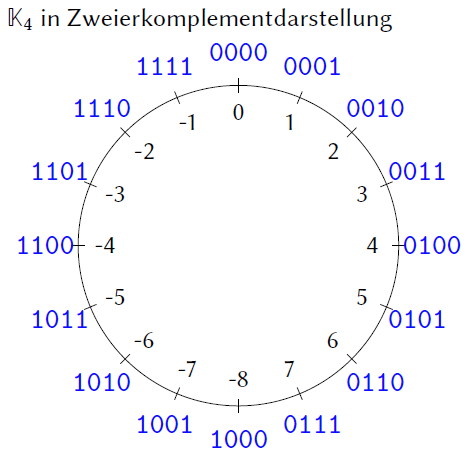
\includegraphics[scale=0.35]{../topics/codierung/ZK_K4}
	\end{figure}

	\begin{exampleblock}{Frage}
		Wie sieht $\nK_5$ aus?
	\end{exampleblock}
\end{frame}

\begin{frame}{Zweierkomplement} % TODO nötig?
    Das Zweierkomplement ist eine Möglichkeit, negative Zahlen binär darzustellen. Im Vergleich zu anderen Darstellungsarten ist es besonders vorteilhaft bei arithmetischen Rechnungen mit Hardware \textit{(mehr dazu in Technischer Informatik)}.
\end{frame}

\begin{frame}{Zweierkomplement}
	\begin{block}{Def.: $\text{Zkpl}_\ell$}
		Die Zweierkomplementdarstellung $ \text{Zkpl}_\ell: \nK \to \set{\texttt{0}, \texttt{1}}^\ell$ der Länge $\ell$:
		$$\text{Zkpl}_\ell(x) = \begin{cases} 0 \text{bin}_{l-1}(x) & \text{falls } x \geq 0 \\ 1 \text{bin}_{l-1}(2^{l-1}+x) & \text{falls } x < 0\end{cases}$$
		Äquivalent:
		$$\text{Zkpl}_\ell(x) = \begin{cases} \text{bin}_{l}(x) & \text{, falls } x \geq 0 \\ \text{bin}_{l}(2^{l}+x) & \text{, falls } x < 0\end{cases}$$
		wobei
		\[
			\text{bin} \colon \nZ_{2^{\ell}} \to \{\texttt{0},\texttt{1}\}^{\ell}, n \mapsto \texttt{0}^{\ell- |\text{Repr}_2(n)|} \text{Repr}_2(n) 
		\]
	\end{block}
\end{frame}
\subsection{Trick}
\begin{frame}{Zweierkomplement}
	\begin{exampleblock}{Ein Trick}
		Zum ``intuitiven'' Berechnen des Zweierkomplement können wir so vorgehen (für $x < 0$):
		\begin{enumerate}
			\item Binärdarstellung von $|x|$ berechnen: $\text{Repr}_2(|x|)$
			\item Mit führenden Nullen auffüllen bis zur Länge $\ell$
			\item Alle binären Ziffern negieren
			\item 1 addieren
		\end{enumerate}
	\end{exampleblock}

	\begin{exampleblock}{Beispiel}
		$$\text{Zkpl}_4(-2): 2 \rightarrow 10 \rightarrow 0010 \rightarrow 1101 \rightarrow 1110 = \text{Zkpl}_4(-2)$$
	\end{exampleblock}
\end{frame}
\subsection{Aufgabe}
\begin{frame}{Zweierkomplement}
	\begin{exampleblock}{Aufgaben}
	Berechne
		\begin{itemize}
			\item $\text{Zkpl}_5(0) \only<2->{= 00000}$ \\
			\item $\text{Zkpl}_5(2) \only<3->{= 00010}$ \\
			\item $\text{Zkpl}_5(15) \only<4->{= 01111}$ \\
			\item $\text{Zkpl}_5(-1) \only<5->{= 11111} $\\
			\item $\text{Zkpl}_5(-6) \only<6->{= 11010} $\\
			\item $\text{Zkpl}_5(-16) \only<7->{= 10000}$
		\end{itemize}
	\end{exampleblock}
\end{frame}

\begin{frame}{Darstellung von Zahlen}
    \begin{exampleblock}{Aufgabe}
    	Es seien die Wörter $u := \texttt{10010}, v := \texttt{01011}$ aus $Z_2^*$.
    	\begin{enumerate}
     		\item Gib die Dezimaldarstellung an, die $u$ und $v$ als Binärdarstellung haben. Gib die Binärdarstellung von $u+v=:w \in Z_2^*$ an.
    		\item Gib den Dezimalwert der Zkpl-Interpretation von $u, v, w$ an, also $\text{Num}_{Zkpl}(x)$ für $x\in \set{u,v,w}$.
    		\item Ist $w$ die Zweierkomplementdarstellung der Summe der Zahlen mit den Zweierkomplementdarstellungen $u$ und $v$?
  		\end{enumerate}
    \end{exampleblock}
\end{frame}
	
\begin{frame}
    \begin{block}{Lösung}
    	\begin{enumerate}
     		\item $\text{Num}_2(u)=18, \text{Num}_2(v)=11, \text{Num}_2(w) = \text{Num}_2(u)+\text{Num}_2(v)=29, w=\texttt{11101}$
    		\pause \item $\text{Num}_{Zkpl}(u)=-14, \text{Num}_{Zkpl}(v)=\text{Num}_2(v)=11, \text{Num}_{Zkpl}(w)=-3$
    		\pause \item Ja, denn $-14+11=-3$.
  		\end{enumerate}
    \end{block}
\end{frame}


% \begin{frame}{ZK: Einfache Berechnung}
% 	Die einzelnen Schritte können wir auch formal angeben:\\
% 	(Wir operieren jeweils auf Wörtern aus $\{0, 1\}^* = Z_2^*$) \\[0.5em]
% 	1. Binärdarstellung von $\setsize{x}$ berechnen: $Repr_2(\setsize{\cdot})$ \\
% 	2. Mit führenden Nullen auffüllen bis zur Länge $\ell$\\ \pause
% 	\begin{align*}
% 		Fill_\ell : Z_2^m &\to Z_2^\ell \qquad (m \le \ell) \\ \visible<3-> {
% 		w &\mapsto \begin{cases}
% 		0^\ell & w = \varepsilon \\
% 		Fill_{\ell-1}(w') \cdot \mu & w = w' \cdot \mu, w' \in Z_2^*, \mu \in Z_2
% 		\end{cases} \\
% 		&\text{oder deutlich einfacher} \\
% 		w &\mapsto \begin{cases}
% 		w & \setsize{w} = \ell \\
% 		Fill_\ell(0w) & \text{sonst}
% 		\end{cases} \\
% 	}
% 	\end{align*}
% 	\pause[4] 3. / 4. Analog %TODO
% \end{frame}

\section{Homomorphismen}

% \begin{frame}
% 	\textbf{Übersetzung:} Bedeutungserhaltende Abbildung \\[0.5em] \pause
% 	\textbf{Codierung:} Injektive Übersetzung \\ \pause
% 	Es reicht eine injektive Abbildung: Dann können wir für jedes $f(w)$ eindeutig das erzeugende $w$ angeben und somit die Bedeutung von $f(w)$ als die Bedeutung von $w$ festlegen. \\[1em]
	
% 	\pause
% 	\emph{Beliebige }Codierungen zu speichern ist sehr aufwendig, bei unendlichem Definitionsbereich sogar unmöglich.\\
% 	Also bringen wir etwas Struktur ins Spiel!
% \end{frame}

% \begin{frame}{Homomorphismen}
% 	Ein Homomorphismus ist eine strukturerhaltende Abbildung. \\
% 	\begin{align*}
% 		\Phi : A &\to B \\
% 		\text{ mit } \forall a \in A, b \in B: \Phi(a \; \square \; b) &= \Phi(a) \; \triangle \; \Phi(b)
% 	\end{align*} 
% \end{frame}
\subsection{Definitionen und alles}
\begin{frame}{Homomorphismen}
	\begin{block}{Def.: Homomorphismus}
		Ein \textbf{Homomorphismus} ist eine strukturerhaltende Abbildung. Wir betrachten Homomorphismen auf Wörtern, dabei muss die Konkatenation erhalten werden.\\
		Seien $A, B$ Alphabete, dann ist Abbildung $h: A^* \to B^*$ ein \textbf{Homomorphismus}, wenn
		$$ \forall\ x, y\in A^* : h(x \cdot y) = h(x) \cdot h(y) $$
	\end{block}
	
	\begin{exampleblock}{Beispiel}
		Sei $h$ ein Homomorphismus mit $h(a) = 2, h(b) = 3$. \\
		Dann gilt $h(aba) = h(a) \cdot h(b) \cdot h(a) = 232 $
	\end{exampleblock}
\end{frame}

\begin{frame}{Homomorphismen}
	\begin{exampleblock}{Aufgabe}
		Gegeben sei die folgende Abbildung über dem Alphabet $A:=\set{a, b, c, \dots, z}$:
		\begin{align*}
			R(\varepsilon) &= \varepsilon,\\
			\text{für alle } w \in A^* gilt: R(wx) &= x \cdot R(w).
		\end{align*}
		\begin{enumerate}
			\item Ist $R$ ein Homomorphismus?
			\item \only<2->{Gib ein Alphabet $A'$ an, sodass $R$ ein Homomorphismus ist.}
		\end{enumerate}
	\end{exampleblock}

	\begin{block}{Lösung}
		\begin{enumerate}
			\item \only<2->{$R$ ist kein Homomorphismus, denn $R(a \cdot b) = ba \neq ab = R(a) \cdot R(b)$.}
			\item \only<3->{$R$ ist ein Homomorphismus, wenn $\setsize{A'}=1$.}
		\end{enumerate}
	\end{block}
\end{frame}

% \begin{frame}{Homomorphismen konstruieren}
% 	Wir können uns aber aus einer Abbildung der einzelnen Zeichen einen Homomorphismus auf Wörtern konstruieren.
% 	\begin{Definition}
% 		Sei $f: A \to B^*,$ \pause definiere $f^{**}:A^* \to B^*$ als
% 		\begin{align*}
% 		f^{**}(\varepsilon) &= \varepsilon  \\
% 		\forall w\in A^*, x\in A: f^{**}(wx) &= f^{**}(w) f(x)       
% 		\end{align*}
% 	\end{Definition}

% 	$f^{**}$ ist der durch $f$ \textbf{induzierte} Homomorphismus.
% \end{frame}

\begin{frame}{Homomorphismen}
	\begin{block}{$\varepsilon$-freier Homomorphismus}
		Ein Homomorphismus heißt \textbf{$\mathbf{\varepsilon}$-frei}, wenn für jedes $\ x\in A$ gilt:
		$$ h(x) \neq \varepsilon. $$
	\end{block}

	\begin{exampleblock}{Vorteil}
		\pause Es gehen keine Informationen verloren:\\
		\begin{itemize}
			\item Betrachte $h: \set{a,b}^* \to \set{0,1}^*$ mit $h(a)=001, h(b)=\varepsilon$
			\item Für welches $w$ gilt $h(w)=001$?
			\item Klar: in $w$ muss ein $a$ sein, aber wie viele $b$s?
		\end{itemize}
	\end{exampleblock}
\end{frame}

\begin{frame}{Homomorphismen}
	\begin{exampleblock}{Wann gehen noch Informationen verloren?}
		\begin{itemize}
			\item Betrachte $h: \set{a, b, c}^* \to \set{0,1}^*$ mit $h(a)=0, h(b)=1, h(c)=10$
			\item Für welches $w$ gilt $h(w)=10$?
			\item \pause Für $w=ba$ und $w=c$
		\end{itemize}
	\end{exampleblock}
	\pause
	\begin{block}{Def.: Präfixfreier Homomorphismus}
		Sei $h: A^* \to B^* $ ein Homomorphismus. h heißt \textbf{präfixfrei}, wenn für
		keine zwei verschiedenen Symbole $x_1,x_2\in A$ gilt: $h(x_1)$
		ist ein Präfix von $h(x_2)$.
	\end{block}
	\begin{exampleblock}{Beispiele}
		\begin{itemize}
			\item $h(a)=001, h(b)=1101$ ist präfixfrei
			\item $h(a)=01, h(b)=011$ ist nicht präfixfrei 
		\end{itemize}
	\end{exampleblock}
\end{frame}

\begin{frame}{Homomorphismen}
	\begin{exampleblock}{Beobachtung}
		Präfixfreie Homomorphismen sind $\varepsilon-$frei
	\end{exampleblock}

	\begin{block}{Def.: Codierung}
		Präfixfreie Homomorphismen sind injektiv. Das wollen wir \textbf{Codierungen} nennen.
	\end{block}

	\begin{exampleblock}{Beobachtung}
		Präfixfreie Codes kann man einfach decodieren\footnote{Das liegt daran, dass zu injektiven Abbildungen  Umkehrabbildung existieren}:
		\[
		u(w) = 
		\begin{cases}
		\varepsilon, & \text{ falls } w=\varepsilon\\
		x\,u(w'), & \text{ falls } w=h(x)w' \text{ für ein } x\in A \\
		\bot,  & \text{ sonst }\\
		\end{cases}
		\]
	\end{exampleblock}
\end{frame}

\section{Huffman-Codierung}
\subsection{Definition}
% \begin{frame}
% 	Kann man mit einer Codierung die benötigte Anzahl der Zeichen für ein Wort reduzieren und trotzdem den Sinn erhalten?\\[0.5em]
% 	\pause
% 	Natürlich geht das (manchmal), dieses Verfahren ist überall im Einsatz:\\
% 	Komprimierung!
% \end{frame}

\begin{frame}{Huffman-Codierung}
	\textbf{Ziel}: möglichst kurze, präfixfreie Codierungen für beliebige Wörter.
	\pause
	\begin{exampleblock}{}
		Eine Huffman-Codierung ist ein präfixfreier (und demnach einfach zu decodierenden) Homomorphismus, bei der die Codierung eines Zeichens umso länger wird, je seltener das Zeichen vorkommt.
	
		Die Huffman-Codierung für ein Wort ist dabei nicht eindeutig, wie wir gleich im Konstruktionsverfahren sehen werden.
	\end{exampleblock}
	% \begin{block}{Lemma}
	% 	Unter allen präfixfreien Codes führen Huffman-Codes zu kürzesten Codierungen
	% 	\textbf{des Wortes, für das die Huffman-Codierung konstruiert wurde.}
	% \end{block}
\end{frame}
\begin{frame}
	\begin{block}{Nützliche (informelle) Definitionen zu Bäumen}
		\begin{itemize}
			\item \textbf{Baum}: besteht aus Knoten, die über Kanten miteinander verbunden sind
			\item \textbf{Wurzel}: Knoten, von dem aus alle anderen Knoten erreichbar sind
			\item \textbf{Blatt}: Ein Knoten ohne ausgehende Kanten
			\item \textbf{Innerer Knoten}: Alle Knoten, die keine Blätter sind
		\end{itemize}
	\end{block}
\end{frame}

\begin{frame}{Huffman-Codierung}
	\begin{block}{Baum konstruieren (informell)}
		\begin{enumerate}
			\item \textbf{Alle Zeichen} mit ihrer \textbf{Häufigkeit} als Blätter in die unterste Ebene zeichnen.
			\item Jeweils zwei Knoten/Bäume (nicht unbeding Blätter!) mit den \textbf{geringsten Häufigkeiten} verbinden, indem man ihnen eine gemeinsame Wurzel gibst, die die Summe der Häufigkeiten erhält.
			\item Fortfahren, bis nur noch \textbf{ein Baum} übrig ist.
			\item Die linken Äste jeweils mit \bzero \ beschriften, die rechten Äste mit \bone.
			\item Die Codierung einzelner Zeichen kann man entlang der Pfade von der Wurzel zum jeweiligen Zeichen ablesen.
		\end{enumerate}
	\end{block}
	\begin{exampleblock}{Am Beispiel}
		Codiere das Wort $w= cabadcdaac $
	\end{exampleblock}
\end{frame}

\begin{frame}{Huffman-Codierung}
    \begin{block}{Lösung}
    \begin{columns}[T] % align columns
    	\begin{column}{.58\textwidth}
			\begin{figure}[b]
				%\centering
				\begin{tikzpicture}
				[level 1/.style={sibling distance=40mm},
				level 2/.style={sibling distance=20mm},
				level 3/.style={sibling distance=15mm}]
				\node {$10$}
				child {
					node{$6$}
					child{
						node{$3$}
						child{
							node{$1,b$}
							edge from parent node[left] {\bzero}
						}
						child {
							node{$2,d$}
							edge from parent node[right] {\bone}
						}
						edge from parent node[left] {\bzero};
					}
					child{
						node{$3,c$}
						edge from parent node[right] {\bone}
					}
					edge from parent node[left] {\bzero};
				}
				child{
					node{$4,a$}
					edge from parent node[right] {\bone}
				};
				\end{tikzpicture}
			\end{figure}  
		\end{column}
			\hfill
		\begin{column}{.44\textwidth}
			\hfill
			\hfill 
			\vspace*{0.1\linewidth}
			\begin{table}[H]
				\begin{tabular}{c|cccc}
					\hline
					x & a & b & c & d  \\ \hline
					$N_x(w)$  & 4 & 1 & 3 & 2 \\ \hline
					h(x) & 1 & 000 & 01 & 001 \\ \hline 
				\end{tabular}
			\end{table}
		\end{column}
	\end{columns}
    \end{block}
\end{frame}

\begin{frame}{Huffman-Codierung}
	\begin{block}{``Operator'' Huffman-Codierung}
		\begin{enumerate}
			\item Häufigkeiten zählen
			\item Baum konstruieren
			\item Abbildung definieren
			\item Codierung des Wortes
		\end{enumerate}
	\end{block}

	\begin{exampleblock}{Aufgabe}
		Betrachte das Alphabet $A:=\set{a,b,c,d,e}.$
		\begin{enumerate}
			\item Bestimme die Huffman-Codierung $h_1(w)$ des Wortes $w:=bbeacdbbea$. Wie ist $|h_1(w)|?$
			\pause \item Bestimme die Huffman-Codierung $h_2(u)$ mit $u:=a^2 b^4 c^8 d^{16} e^{32}$.
			\pause \item Zerlege $w$ in Zweierblöcke und fasse diese als Zeichen auf. Wie ist nun die Blockcodierung $h_3(w)$? Wie verhält sich $|h_1(w)|$ zu $|h_3(w)|$?
		\end{enumerate}
	\end{exampleblock}
\end{frame}
}

\Stephan{
\section{Darstellung von Zahlen}
\subsection{Num}
\begin{frame}{Von Wörtern zu Zahlen}
	\begin{block}{Def.: $\text{Num}_k$}
		Zu einer Zahlenbasis $k$ definiere die Abbildung $\text{Num}_k : Z_k^* \to \nZ$ 

		\begin{align*}
			\text{Num}_k(\varepsilon) &= 0 \\
			\text{Num}_k(wx) &= k\cdot \text{Num}_k(w) + \text{num}_k(x) \text{ für alle } w\in Z_k^*, x\in Z_k\\[2ex]
			\text{wobei }\text{num}_k(x) &= x \text{ für alle } x \in \set{1,\dots,k-1}
		\end{align*}
	\end{block}
	\pause
	\begin{exampleblock}{Beispiel}
		\begin{align*}
			\text{Num}_2(11) &= 2\cdot \text{Num}_2(1) + \text{num}_2(1) \\
				&= 2\cdot 1 + 1 \\
				&= 3
		\end{align*}
	\end{exampleblock}
\end{frame}

\begin{frame}{Von Wörtern zu Zahlen}
	\begin{exampleblock}{Aufgabe: Berechne die Zahlenwerte von $321_4, B2_{16}$}
	\begin{align*}
	\text{Num}_4(321) &= \visible<2->{ 4\cdot \text{Num}_4(32) + \text{num}_4(1) \\
	&= 4\cdot \left( 4\cdot \text{Num}_4(3) + \text{num}_4(2) \right) + \text{num}_4(1) \\
	&= 4^2\cdot \text{num}_4(3) + 4 \cdot \text{num}_4(2) + \text{num}_4(1) \\
	&= 57 \\}
	\visible<3->{\text{Num}_{16}(B2) &=} \visible<4->{ 16 \cdot \text{Num}_{16}(B) + \text{num}_{16}(2) \\
	&= 16\cdot 11 + 2 \\
	&= 178}
	\end{align*}
	\end{exampleblock}
	\visible<5->{
	\begin{exampleblock}{Aufgabe}
		$\text{Num}_2(1), \text{ Num}_2(11), \text{ Num}_2(111), \text{ Num}_2(1111)$\\
		Was gilt allgemein für $\text{Num}_2(1^m)$ für $m \in \nN_0$?
	\end{exampleblock}}
\end{frame}

\subsection{mod und div}
\begin{frame}{Division und Modulo}
	\begin{block}{\div und \mod}
		$ x \div y$ ist die ganzzahlige Division von x durch y.\\
		$ x \mod y$ liefert den Rest dieser Division.
	\end{block} 
	\begin{block}{Beobachtung}
		$$ 0 \leq (x \mod y ) < y$$
	\end{block}
	\begin{block}{Lemma}
		$$ x = y \cdot (x \div y ) + \left( x \mod y \right)$$ 
	\end{block}
\end{frame}

\begin{frame}{Division und Modulo}
	\begin{exampleblock}{Beispiel}
		\begin{table}[h!]
			\begin{tabular}{c|cc}
				& $x\div y$ & $x\mod y$ \\ \hline
				$x=2,y=3$ \only<2-|handout:0>{&  0 & 2 } \only<1>{&&}\\
				$x=5 ,y=2$ \only<3-|handout:0>{ & 2 & 1 } \only<1-2>{&&} \\
				$x=8,y=2$ \only<4-|handout:0>{ & 4 & 0 } \only<1-3>{&&} \\	
			\end{tabular}
		\end{table}
	\end{exampleblock}
\end{frame}

\begin{frame}{Division und Modulo}
	\begin{exampleblock}{Aufgabe}
		Fülle die folgende Tabelle aus
		\begin{table}[h!]
		\begin{tabular}{c|cccccccccccc}
			$x$ & 0 & 1 & 2 & 3 & 4 & 5 & 6 & 7 & 8 & 9 & 10 & 11 \\ \hline
			$x\div 4 $ & \only<1>{ &&&&&&&&&&} \only<2-|handout:0>{0 & 0 & 0 & 0 & 1 & 1 & 1 & 1 & 2 & 2 & 2 & 2}\\
			$4\left( x\div 4\right) $ & \only<1-2>{&&&&&&&&&&} \only<3-|handout:0>{0&0&0&0&4&4&4&4&8&8&8&8}\\
			$x\mod 4$ & \only<1-3>{&&&&&&&&&&} \only<4-|handout:0>{0&1&2&3&0&1&2&3&0&1&2&3}
		\end{tabular}
		\end{table}
	\end{exampleblock}
\end{frame}

\subsection{Repr}
\begin{frame}{Repräsentation}
	\begin{block}{Def.: $Repr_k$}
		\begin{align*}
			Repr_k : \; &\nN_0 \to Z_k  \\
			n&\mapsto \begin{cases} repr_k(n) & \text{, falls } n<k \\
				Repr_k\left( n\div k \right) \cdot repr_k\left( n \mod 	k \right) & \text{, falls } n\geq k 
			\end{cases}\\
			\text{Wobei für alle } &x \in \nZ_k : \text{repr}_k(x) = x.
		\end{align*}
	\end{block}
	\pause
	\begin{exampleblock}{Aufgabe}
		Berechne folgende Darstellungen:\\
		$Repr_2(42) = \pause 101010$ \\
		$Repr_4(42) = \pause 222$ \\
		$Repr_8(42) = \pause 52$ \\
		$Repr_{16}(42) = \pause 2A$
	\end{exampleblock}
\end{frame}

% \begin{frame}{Beispiel: Lösung}
% 	\begin{align*}
% 		Repr_8(42) &= Repr_8(42 \div 8) \cdot repr_8(42 \mod 8) \\
% 		&= Repr_8(5) \cdot repr_8(2)\\
% 		&= repr_8(5) \cdot 2\\
% 		&= 5 \cdot 2\\
% 		&= 52_8
% 	\end{align*}
% \end{frame}

\begin{frame}{Repräsentation}
	\begin{block}{Korrolar}
		$Repr_k(n)$ ist das kürzeste Wort $w\in Z_k^\ast$ mit $Num_k(w)=n$, also 
		$$ Num_k\left( Repr_k(n)\right) = n $$
	\end{block}

	\begin{alertblock}{Anmerkung}
		Im Allgemeinen  $Repr_k\left(Num_k(w)\right) \neq w $, da überflüssige Nullen wegfallen.
	\end{alertblock}
	
	\Stephan{
	\begin{exampleblock}{Schaubild}
		s. Tafel
	\end{exampleblock}
	}
	%TODO
	% \begin{exampleblock}{Zusammenhang}
	% 	\begin{tikzpicture}[
 %    		node distance=2mm,
 %    		>=stealth, auto,
	% 		every state/.style={draw=none, inner sep=0pt}
 %                		]

	% 			\node[state] (q1) {Dezimaldarstellung};
	% 			\node[state] (q2) [above right=of q1] {$\text{Repr}_k$};
	% 			\node[state] (q3) [below right=of q2] {k-äre Darstellung};
	% 			\node[state] (q4) [below right=of q1] {$\text{Num}_k$};

 %    		\begin{scope}[bend left]%
	% 	\path[->]   (q1) edge node {c} (q2)
 %            		(q2) edge node {c} (q3)
 %            		(q3) edge node {c} (q4)
 %            		(q4) edge node {c} (q1);
 %    		\end{scope}
	% 	\end{tikzpicture}
	% \end{exampleblock}	 
\end{frame}

\subsection{Zweierkomplement}
\begin{frame}{Ein asymetrischer Zahlenbereich}
	\[
	\nK_{\ell} := \{ x\in \nZ\mid -2^{\ell-1} \leq x \leq 2^{\ell-1} -1 \} \;.
	\]
	\\[0.2cm]
	
	\begin{figure}
		\centering
		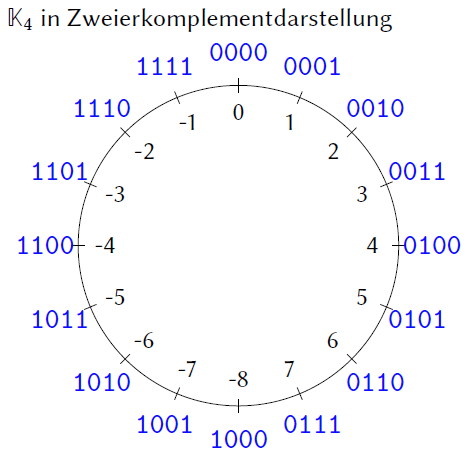
\includegraphics[scale=0.35]{../topics/codierung/ZK_K4}
	\end{figure}

	\begin{exampleblock}{Frage}
		Wie sieht $\nK_5$ aus?
	\end{exampleblock}
\end{frame}

\begin{frame}{Zweierkomplement} % TODO nötig?
    Das Zweierkomplement ist eine Möglichkeit, negative Zahlen binär darzustellen. Im Vergleich zu anderen Darstellungsarten ist es besonders vorteilhaft bei arithmetischen Rechnungen mit Hardware \textit{(mehr dazu in Technischer Informatik)}.
\end{frame}

\begin{frame}{Zweierkomplement}
	\begin{block}{Def.: $\text{Zkpl}_\ell$}
		Die Zweierkomplementdarstellung $ \text{Zkpl}_\ell: \nK \to \set{\texttt{0}, \texttt{1}}^\ell$ der Länge $\ell$:
		$$\text{Zkpl}_\ell(x) = \begin{cases} 0 \text{bin}_{l-1}(x) & \text{falls } x \geq 0 \\ 1 \text{bin}_{l-1}(2^{l-1}+x) & \text{falls } x < 0\end{cases}$$
		Äquivalent:
		$$\text{Zkpl}_\ell(x) = \begin{cases} \text{bin}_{l}(x) & \text{, falls } x \geq 0 \\ \text{bin}_{l}(2^{l}+x) & \text{, falls } x < 0\end{cases}$$
		wobei
		\[
			\text{bin} \colon \nZ_{2^{\ell}} \to \{\texttt{0},\texttt{1}\}^{\ell}, n \mapsto \texttt{0}^{\ell- |\text{Repr}_2(n)|} \text{Repr}_2(n) 
		\]
	\end{block}
\end{frame}
\subsection{Trick}
\begin{frame}{Zweierkomplement}
	\begin{exampleblock}{Ein Trick}
		Zum ``intuitiven'' Berechnen des Zweierkomplement können wir so vorgehen (für $x < 0$):
		\begin{enumerate}
			\item Binärdarstellung von $|x|$ berechnen: $\text{Repr}_2(|x|)$
			\item Mit führenden Nullen auffüllen bis zur Länge $\ell$
			\item Alle binären Ziffern negieren
			\item 1 addieren
		\end{enumerate}
	\end{exampleblock}

	\begin{exampleblock}{Beispiel}
		$$\text{Zkpl}_4(-2): 2 \rightarrow 10 \rightarrow 0010 \rightarrow 1101 \rightarrow 1110 = \text{Zkpl}_4(-2)$$
	\end{exampleblock}
\end{frame}
\subsection{Aufgabe}
\begin{frame}{Zweierkomplement}
	\begin{exampleblock}{Aufgaben}
	Berechne
		\begin{itemize}
			\item $\text{Zkpl}_5(0) \only<2->{= 00000}$ \\
			\item $\text{Zkpl}_5(2) \only<3->{= 00010}$ \\
			\item $\text{Zkpl}_5(15) \only<4->{= 01111}$ \\
			\item $\text{Zkpl}_5(-1) \only<5->{= 11111} $\\
			\item $\text{Zkpl}_5(-6) \only<6->{= 11010} $\\
			\item $\text{Zkpl}_5(-16) \only<7->{= 10000}$
		\end{itemize}
	\end{exampleblock}
\end{frame}

\begin{frame}{Darstellung von Zahlen}
    \begin{exampleblock}{Aufgabe}
    	Es seien die Wörter $u := \texttt{10010}, v := \texttt{01011}$ aus $Z_2^*$.
    	\begin{enumerate}
     		\item Gib die Dezimaldarstellung an, die $u$ und $v$ als Binärdarstellung haben. Gib die Binärdarstellung von $u+v=:w \in Z_2^*$ an.
    		\item Gib den Dezimalwert der Zkpl-Interpretation von $u, v, w$ an, also $\text{Num}_{Zkpl}(x)$ für $x\in \set{u,v,w}$.
    		\item Ist $w$ die Zweierkomplementdarstellung der Summe der Zahlen mit den Zweierkomplementdarstellungen $u$ und $v$?
  		\end{enumerate}
    \end{exampleblock}
\end{frame}
	
\begin{frame}
    \begin{block}{Lösung}
    	\begin{enumerate}
     		\item $\text{Num}_2(u)=18, \text{Num}_2(v)=11, \text{Num}_2(w) = \text{Num}_2(u)+\text{Num}_2(v)=29, w=\texttt{11101}$
    		\pause \item $\text{Num}_{Zkpl}(u)=-14, \text{Num}_{Zkpl}(v)=\text{Num}_2(v)=11, \text{Num}_{Zkpl}(w)=-3$
    		\pause \item Ja, denn $-14+11=-3$.
  		\end{enumerate}
    \end{block}
\end{frame}


% \begin{frame}{ZK: Einfache Berechnung}
% 	Die einzelnen Schritte können wir auch formal angeben:\\
% 	(Wir operieren jeweils auf Wörtern aus $\{0, 1\}^* = Z_2^*$) \\[0.5em]
% 	1. Binärdarstellung von $\setsize{x}$ berechnen: $Repr_2(\setsize{\cdot})$ \\
% 	2. Mit führenden Nullen auffüllen bis zur Länge $\ell$\\ \pause
% 	\begin{align*}
% 		Fill_\ell : Z_2^m &\to Z_2^\ell \qquad (m \le \ell) \\ \visible<3-> {
% 		w &\mapsto \begin{cases}
% 		0^\ell & w = \varepsilon \\
% 		Fill_{\ell-1}(w') \cdot \mu & w = w' \cdot \mu, w' \in Z_2^*, \mu \in Z_2
% 		\end{cases} \\
% 		&\text{oder deutlich einfacher} \\
% 		w &\mapsto \begin{cases}
% 		w & \setsize{w} = \ell \\
% 		Fill_\ell(0w) & \text{sonst}
% 		\end{cases} \\
% 	}
% 	\end{align*}
% 	\pause[4] 3. / 4. Analog %TODO
% \end{frame}

\section{Homomorphismen}

% \begin{frame}
% 	\textbf{Übersetzung:} Bedeutungserhaltende Abbildung \\[0.5em] \pause
% 	\textbf{Codierung:} Injektive Übersetzung \\ \pause
% 	Es reicht eine injektive Abbildung: Dann können wir für jedes $f(w)$ eindeutig das erzeugende $w$ angeben und somit die Bedeutung von $f(w)$ als die Bedeutung von $w$ festlegen. \\[1em]
	
% 	\pause
% 	\emph{Beliebige }Codierungen zu speichern ist sehr aufwendig, bei unendlichem Definitionsbereich sogar unmöglich.\\
% 	Also bringen wir etwas Struktur ins Spiel!
% \end{frame}

% \begin{frame}{Homomorphismen}
% 	Ein Homomorphismus ist eine strukturerhaltende Abbildung. \\
% 	\begin{align*}
% 		\Phi : A &\to B \\
% 		\text{ mit } \forall a \in A, b \in B: \Phi(a \; \square \; b) &= \Phi(a) \; \triangle \; \Phi(b)
% 	\end{align*} 
% \end{frame}
\subsection{Definitionen und alles}
\begin{frame}{Homomorphismen}
	\begin{block}{Def.: Homomorphismus}
		Ein \textbf{Homomorphismus} ist eine strukturerhaltende Abbildung. Wir betrachten Homomorphismen auf Wörtern, dabei muss die Konkatenation erhalten werden.\\
		Seien $A, B$ Alphabete, dann ist Abbildung $h: A^* \to B^*$ ein \textbf{Homomorphismus}, wenn
		$$ \forall\ x, y\in A^* : h(x \cdot y) = h(x) \cdot h(y) $$
	\end{block}
	
	\begin{exampleblock}{Beispiel}
		Sei $h$ ein Homomorphismus mit $h(a) = 2, h(b) = 3$. \\
		Dann gilt $h(aba) = h(a) \cdot h(b) \cdot h(a) = 232 $
	\end{exampleblock}
\end{frame}

\begin{frame}{Homomorphismen}
	\begin{exampleblock}{Aufgabe}
		Gegeben sei die folgende Abbildung über dem Alphabet $A:=\set{a, b, c, \dots, z}$:
		\begin{align*}
			R(\varepsilon) &= \varepsilon,\\
			\text{für alle } w \in A^* gilt: R(wx) &= x \cdot R(w).
		\end{align*}
		\begin{enumerate}
			\item Ist $R$ ein Homomorphismus?
			\item \only<2->{Gib ein Alphabet $A'$ an, sodass $R$ ein Homomorphismus ist.}
		\end{enumerate}
	\end{exampleblock}

	\begin{block}{Lösung}
		\begin{enumerate}
			\item \only<2->{$R$ ist kein Homomorphismus, denn $R(a \cdot b) = ba \neq ab = R(a) \cdot R(b)$.}
			\item \only<3->{$R$ ist ein Homomorphismus, wenn $\setsize{A'}=1$.}
		\end{enumerate}
	\end{block}
\end{frame}

% \begin{frame}{Homomorphismen konstruieren}
% 	Wir können uns aber aus einer Abbildung der einzelnen Zeichen einen Homomorphismus auf Wörtern konstruieren.
% 	\begin{Definition}
% 		Sei $f: A \to B^*,$ \pause definiere $f^{**}:A^* \to B^*$ als
% 		\begin{align*}
% 		f^{**}(\varepsilon) &= \varepsilon  \\
% 		\forall w\in A^*, x\in A: f^{**}(wx) &= f^{**}(w) f(x)       
% 		\end{align*}
% 	\end{Definition}

% 	$f^{**}$ ist der durch $f$ \textbf{induzierte} Homomorphismus.
% \end{frame}

\begin{frame}{Homomorphismen}
	\begin{block}{$\varepsilon$-freier Homomorphismus}
		Ein Homomorphismus heißt \textbf{$\mathbf{\varepsilon}$-frei}, wenn für jedes $\ x\in A$ gilt:
		$$ h(x) \neq \varepsilon. $$
	\end{block}

	\begin{exampleblock}{Vorteil}
		\pause Es gehen keine Informationen verloren:\\
		\begin{itemize}
			\item Betrachte $h: \set{a,b}^* \to \set{0,1}^*$ mit $h(a)=001, h(b)=\varepsilon$
			\item Für welches $w$ gilt $h(w)=001$?
			\item Klar: in $w$ muss ein $a$ sein, aber wie viele $b$s?
		\end{itemize}
	\end{exampleblock}
\end{frame}

\begin{frame}{Homomorphismen}
	\begin{exampleblock}{Wann gehen noch Informationen verloren?}
		\begin{itemize}
			\item Betrachte $h: \set{a, b, c}^* \to \set{0,1}^*$ mit $h(a)=0, h(b)=1, h(c)=10$
			\item Für welches $w$ gilt $h(w)=10$?
			\item \pause Für $w=ba$ und $w=c$
		\end{itemize}
	\end{exampleblock}
	\pause
	\begin{block}{Def.: Präfixfreier Homomorphismus}
		Sei $h: A^* \to B^* $ ein Homomorphismus. h heißt \textbf{präfixfrei}, wenn für
		keine zwei verschiedenen Symbole $x_1,x_2\in A$ gilt: $h(x_1)$
		ist ein Präfix von $h(x_2)$.
	\end{block}
	\begin{exampleblock}{Beispiele}
		\begin{itemize}
			\item $h(a)=001, h(b)=1101$ ist präfixfrei
			\item $h(a)=01, h(b)=011$ ist nicht präfixfrei 
		\end{itemize}
	\end{exampleblock}
\end{frame}

\begin{frame}{Homomorphismen}
	\begin{exampleblock}{Beobachtung}
		Präfixfreie Homomorphismen sind $\varepsilon-$frei
	\end{exampleblock}

	\begin{block}{Def.: Codierung}
		Präfixfreie Homomorphismen sind injektiv. Das wollen wir \textbf{Codierungen} nennen.
	\end{block}

	\begin{exampleblock}{Beobachtung}
		Präfixfreie Codes kann man einfach decodieren\footnote{Das liegt daran, dass zu injektiven Abbildungen  Umkehrabbildung existieren}:
		\[
		u(w) = 
		\begin{cases}
		\varepsilon, & \text{ falls } w=\varepsilon\\
		x\,u(w'), & \text{ falls } w=h(x)w' \text{ für ein } x\in A \\
		\bot,  & \text{ sonst }\\
		\end{cases}
		\]
	\end{exampleblock}
\end{frame}

\section{Huffman-Codierung}
\subsection{Definition}
% \begin{frame}
% 	Kann man mit einer Codierung die benötigte Anzahl der Zeichen für ein Wort reduzieren und trotzdem den Sinn erhalten?\\[0.5em]
% 	\pause
% 	Natürlich geht das (manchmal), dieses Verfahren ist überall im Einsatz:\\
% 	Komprimierung!
% \end{frame}

\begin{frame}{Huffman-Codierung}
	\textbf{Ziel}: möglichst kurze, präfixfreie Codierungen für beliebige Wörter.
	\pause
	\begin{exampleblock}{}
		Eine Huffman-Codierung ist ein präfixfreier (und demnach einfach zu decodierenden) Homomorphismus, bei der die Codierung eines Zeichens umso länger wird, je seltener das Zeichen vorkommt.
	
		Die Huffman-Codierung für ein Wort ist dabei nicht eindeutig, wie wir gleich im Konstruktionsverfahren sehen werden.
	\end{exampleblock}
	% \begin{block}{Lemma}
	% 	Unter allen präfixfreien Codes führen Huffman-Codes zu kürzesten Codierungen
	% 	\textbf{des Wortes, für das die Huffman-Codierung konstruiert wurde.}
	% \end{block}
\end{frame}
\begin{frame}
	\begin{block}{Nützliche (informelle) Definitionen zu Bäumen}
		\begin{itemize}
			\item \textbf{Baum}: besteht aus Knoten, die über Kanten miteinander verbunden sind
			\item \textbf{Wurzel}: Knoten, von dem aus alle anderen Knoten erreichbar sind
			\item \textbf{Blatt}: Ein Knoten ohne ausgehende Kanten
			\item \textbf{Innerer Knoten}: Alle Knoten, die keine Blätter sind
		\end{itemize}
	\end{block}
\end{frame}

\begin{frame}{Huffman-Codierung}
	\begin{block}{Baum konstruieren (informell)}
		\begin{enumerate}
			\item \textbf{Alle Zeichen} mit ihrer \textbf{Häufigkeit} als Blätter in die unterste Ebene zeichnen.
			\item Jeweils zwei Knoten/Bäume (nicht unbeding Blätter!) mit den \textbf{geringsten Häufigkeiten} verbinden, indem man ihnen eine gemeinsame Wurzel gibst, die die Summe der Häufigkeiten erhält.
			\item Fortfahren, bis nur noch \textbf{ein Baum} übrig ist.
			\item Die linken Äste jeweils mit \bzero \ beschriften, die rechten Äste mit \bone.
			\item Die Codierung einzelner Zeichen kann man entlang der Pfade von der Wurzel zum jeweiligen Zeichen ablesen.
		\end{enumerate}
	\end{block}
	\begin{exampleblock}{Am Beispiel}
		Codiere das Wort $w= cabadcdaac $
	\end{exampleblock}
\end{frame}

\begin{frame}{Huffman-Codierung}
    \begin{block}{Lösung}
    \begin{columns}[T] % align columns
    	\begin{column}{.58\textwidth}
			\begin{figure}[b]
				%\centering
				\begin{tikzpicture}
				[level 1/.style={sibling distance=40mm},
				level 2/.style={sibling distance=20mm},
				level 3/.style={sibling distance=15mm}]
				\node {$10$}
				child {
					node{$6$}
					child{
						node{$3$}
						child{
							node{$1,b$}
							edge from parent node[left] {\bzero}
						}
						child {
							node{$2,d$}
							edge from parent node[right] {\bone}
						}
						edge from parent node[left] {\bzero};
					}
					child{
						node{$3,c$}
						edge from parent node[right] {\bone}
					}
					edge from parent node[left] {\bzero};
				}
				child{
					node{$4,a$}
					edge from parent node[right] {\bone}
				};
				\end{tikzpicture}
			\end{figure}  
		\end{column}
			\hfill
		\begin{column}{.44\textwidth}
			\hfill
			\hfill 
			\vspace*{0.1\linewidth}
			\begin{table}[H]
				\begin{tabular}{c|cccc}
					\hline
					x & a & b & c & d  \\ \hline
					$N_x(w)$  & 4 & 1 & 3 & 2 \\ \hline
					h(x) & 1 & 000 & 01 & 001 \\ \hline 
				\end{tabular}
			\end{table}
		\end{column}
	\end{columns}
    \end{block}
\end{frame}

\begin{frame}{Huffman-Codierung}
	\begin{block}{``Operator'' Huffman-Codierung}
		\begin{enumerate}
			\item Häufigkeiten zählen
			\item Baum konstruieren
			\item Abbildung definieren
			\item Codierung des Wortes
		\end{enumerate}
	\end{block}

	\begin{exampleblock}{Aufgabe}
		Betrachte das Alphabet $A:=\set{a,b,c,d,e}.$
		\begin{enumerate}
			\item Bestimme die Huffman-Codierung $h_1(w)$ des Wortes $w:=bbeacdbbea$. Wie ist $|h_1(w)|?$
			\pause \item Bestimme die Huffman-Codierung $h_2(u)$ mit $u:=a^2 b^4 c^8 d^{16} e^{32}$.
			\pause \item Zerlege $w$ in Zweierblöcke und fasse diese als Zeichen auf. Wie ist nun die Blockcodierung $h_3(w)$? Wie verhält sich $|h_1(w)|$ zu $|h_3(w)|$?
		\end{enumerate}
	\end{exampleblock}
\end{frame}
}

\Kilian{
	\section{Huffman-Codierung}
	\subsection{Definition}
% \begin{frame}
% 	Kann man mit einer Codierung die benötigte Anzahl der Zeichen für ein Wort reduzieren und trotzdem den Sinn erhalten?\\[0.5em]
% 	\pause
% 	Natürlich geht das (manchmal), dieses Verfahren ist überall im Einsatz:\\
% 	Komprimierung!
% \end{frame}

\begin{frame}{Huffman-Codierung}
	\textbf{Ziel}: möglichst kurze, präfixfreie Codierungen für beliebige Wörter.
	\pause
	\begin{exampleblock}{}
		Eine Huffman-Codierung ist ein präfixfreier (und demnach einfach zu decodierenden) Homomorphismus, bei der die Codierung eines Zeichens umso länger wird, je seltener das Zeichen vorkommt.
	
		Die Huffman-Codierung für ein Wort ist dabei nicht eindeutig, wie wir gleich im Konstruktionsverfahren sehen werden.
	\end{exampleblock}
	% \begin{block}{Lemma}
	% 	Unter allen präfixfreien Codes führen Huffman-Codes zu kürzesten Codierungen
	% 	\textbf{des Wortes, für das die Huffman-Codierung konstruiert wurde.}
	% \end{block}
\end{frame}
\begin{frame}
	\begin{block}{Nützliche (informelle) Definitionen zu Bäumen}
		\begin{itemize}
			\item \textbf{Baum}: besteht aus Knoten, die über Kanten miteinander verbunden sind
			\item \textbf{Wurzel}: Knoten, von dem aus alle anderen Knoten erreichbar sind
			\item \textbf{Blatt}: Ein Knoten ohne ausgehende Kanten
			\item \textbf{Innerer Knoten}: Alle Knoten, die keine Blätter sind
		\end{itemize}
	\end{block}
\end{frame}

\begin{frame}{Huffman-Codierung}
	\begin{block}{Baum konstruieren (informell)}
		\begin{enumerate}
			\item \textbf{Alle Zeichen} mit ihrer \textbf{Häufigkeit} als Blätter in die unterste Ebene zeichnen.
			\item Jeweils zwei Knoten/Bäume (nicht unbeding Blätter!) mit den \textbf{geringsten Häufigkeiten} verbinden, indem man ihnen eine gemeinsame Wurzel gibst, die die Summe der Häufigkeiten erhält.
			\item Fortfahren, bis nur noch \textbf{ein Baum} übrig ist.
			\item Die linken Äste jeweils mit \bzero \ beschriften, die rechten Äste mit \bone.
			\item Die Codierung einzelner Zeichen kann man entlang der Pfade von der Wurzel zum jeweiligen Zeichen ablesen.
		\end{enumerate}
	\end{block}
	\begin{exampleblock}{Am Beispiel}
		Codiere das Wort $w= cabadcdaac $
	\end{exampleblock}
\end{frame}

\begin{frame}{Huffman-Codierung}
    \begin{block}{Lösung}
    \begin{columns}[T] % align columns
    	\begin{column}{.58\textwidth}
			\begin{figure}[b]
				%\centering
				\begin{tikzpicture}
				[level 1/.style={sibling distance=40mm},
				level 2/.style={sibling distance=20mm},
				level 3/.style={sibling distance=15mm}]
				\node {$10$}
				child {
					node{$6$}
					child{
						node{$3$}
						child{
							node{$1,b$}
							edge from parent node[left] {\bzero}
						}
						child {
							node{$2,d$}
							edge from parent node[right] {\bone}
						}
						edge from parent node[left] {\bzero};
					}
					child{
						node{$3,c$}
						edge from parent node[right] {\bone}
					}
					edge from parent node[left] {\bzero};
				}
				child{
					node{$4,a$}
					edge from parent node[right] {\bone}
				};
				\end{tikzpicture}
			\end{figure}  
		\end{column}
			\hfill
		\begin{column}{.44\textwidth}
			\hfill
			\hfill 
			\vspace*{0.1\linewidth}
			\begin{table}[H]
				\begin{tabular}{c|cccc}
					\hline
					x & a & b & c & d  \\ \hline
					$N_x(w)$  & 4 & 1 & 3 & 2 \\ \hline
					h(x) & 1 & 000 & 01 & 001 \\ \hline 
				\end{tabular}
			\end{table}
		\end{column}
	\end{columns}
    \end{block}
\end{frame}

\begin{frame}{Huffman-Codierung}
	\begin{block}{``Operator'' Huffman-Codierung}
		\begin{enumerate}
			\item Häufigkeiten zählen
			\item Baum konstruieren
			\item Abbildung definieren
			\item Codierung des Wortes
		\end{enumerate}
	\end{block}

	\begin{exampleblock}{Aufgabe}
		Betrachte das Alphabet $A:=\set{a,b,c,d,e}.$
		\begin{enumerate}
			\item Bestimme die Huffman-Codierung $h_1(w)$ des Wortes $w:=bbeacdbbea$. Wie ist $|h_1(w)|?$
			\pause \item Bestimme die Huffman-Codierung $h_2(u)$ mit $u:=a^2 b^4 c^8 d^{16} e^{32}$.
			\pause \item Zerlege $w$ in Zweierblöcke und fasse diese als Zeichen auf. Wie ist nun die Blockcodierung $h_3(w)$? Wie verhält sich $|h_1(w)|$ zu $|h_3(w)|$?
		\end{enumerate}
	\end{exampleblock}
\end{frame}
}

% \section{Speicher}
% \subsection{Funktionen von Funktionen}

\begin{frame}{Funktionsception: Funktionen von Funktionen}
	\begin{block}{Def.: $B^A$}
		Seien A und B Mengen. Mit $B^A$ bezeichnen wir die Menge aller Abbildungen von $A$ nach $B$, also $$B^A = \set{f \mid f : A \to B }$$
	\end{block}

	\begin{block}{Beobachtung}
		Für endliche Mengen $A$ und $B$ gilt:
		$$|B^A| = |B|^{|A|}$$
	\end{block}
\end{frame}

\begin{frame}{Funktionsception${}^2$: Funktionen als Argument von Funktionen}

	\begin{exampleblock}{Beispiel}
		\small Es sei $M$ eine Menge. Jede Teilmenge $L \subseteq M$ kann man mit einer Abbildung $f_L \colon M \to \set{0,1}$, also einem $f_L \in \set{0,1}^M$ in Beziehung setzen.

		Für die Teilmenge $L \subseteq M$ ist 
		\begin{equation*} 
			f_L \colon M \to \set{0,1}, x \mapsto
			\begin{cases}
				1 & \text{, falls } x \in L \\
				0 & \text{, falls } x \notin L
			\end{cases}
		\end{equation*}
	\end{exampleblock}
\end{frame}

\begin{frame}{Funktionsception${}^2$: Funktionen als Argument von Funktionen}
	\begin{exampleblock}{Beispiel}
		Dann kann man die Vereinigung $\sqcup$ als Abbildung darstellen:
		$$\sqcup \colon \{0,1\}^M \times \{0,1\}^M\to \{0,1\}^M$$
		\pause
		\begin{columns}
			\begin{column}{0.4\textwidth}
				Beispielbild für $A=\{a,c,d\}$ \\ und $B=\{b,c\}$
			\end{column}
			\begin{column}{0.4\textwidth}
				\begin{tabular}{*{4}{>{$}c<{$}}}
					& A & B & A\cup B \\
					x & f_A(x) & f_B(x) & (\sqcup(f_A,f_B))(x) \\
					\hline
					a & 1 & 0 & 1 \\
					b & 0 & 1 & 1 \\
					c & 1 & 1 & 1 \\
					d & 1 & 0 & 1 \\
					e & 0 & 0 & 0 \\
				\end{tabular}
			\end{column}
			\end{columns}	
		\medskip
		\centering Wie könnte nun eine Abbildungsvorschrift aussehen?
	\end{exampleblock}
\end{frame}
\begin{frame}{Funktionsception${}^2$: Funktionen als Argument von Funktionen}
	\begin{exampleblock}{Wie könnte eine Abbildungsvorschrift aussehen?}
	\begin{align*}
		\sqcup\colon \{0,1\}^M \times \{0,1\}^M &\to \{0,1\}^M \\
		(f_A,f_B) &\mapsto (x \mapsto \max(f_A(x),f_B(x))) \\[2ex]
		\text{also }  \sqcup(f_A,f_B) (x) &= \max(f_A(x),f_B(x)) \\
	\end{align*}
	\end{exampleblock}
\end{frame}

\subsection{Speicher}

\begin{frame}{Bits und Bytes}
	\begin{block}{Def.: Bit und Byte}
		Ein \textbf{Bit} ist ein Zeichen des Alphabets $\set{0,1}$. \\
		Ein Wort aus 8 Bits wird \textbf{Byte} genannt. 
	\end{block}
\end{frame}
\begin{frame}{Speicher}
	\begin{block}{Speicher}
		Ein \textbf{Speicher} $m$ bildet Adressen ($Adr$) auf Werte ($Val$) ab.\\
		Also $m \in Val^{Adr}$ bzw. $m \colon Adr \to Val$.
	\end{block}

	\begin{exampleblock}{Dazu sei einiges gesagt:}
		\begin{itemize}
			\item Statt ``Speicher'' trifft es \textbf{aktueller Zustand des Speichers} besser.
			\item Vorstellung als Tabelle. Linke Spalte Adressen, rechte Spalte Werte.
			\item Uns interessiert (noch) nicht die konkrete Realisierung, sondern nur die abstrakte Funktionsweise.
			\item Im Umgang mit Speicher benutzen wir hier nur Zahlen im Binärsystem, d.h.
				$$Adr = 2^k, Val = 2^l \quad k,l \in \nN_+$$
				Bei der \emph{MIMA}: $k=20, l=24$.
		\end{itemize}
	\end{exampleblock}
\end{frame}

\begin{frame}{Speicher - Methoden}
	\begin{block}{Def.: $memread$}
		Gibt im aktuellen Speicherzustand $m$ den Wert an der Adresse $a$ zurück.
		\begin{align*}
			memread : Val^{Adr} \times Adr &\to Val \\
									(m,a) &\mapsto m(a)
	\end{align*}
	\end{block}
\end{frame}

\begin{frame}{Speicher - Methoden}
	\begin{block}{Def.: $memwrite$}
		Speichert einen Wert $v$ in die Adresse $a$.
		\begin{align*}
			memwrite : Val^{Adr} \times Adr \times Val &\to Val^{Adr} \\
			(m,a,v) &\mapsto m' \\
		\end{align*}

		$m'$ ist nun ein neuer Speicherzustand, für den gilt:
		\begin{equation*}
			m'(a') =
				\begin{cases}
					v & \text{, falls } a'=a \\
					m(a') & \text{, sonst}
				\end{cases}
		\end{equation*}
		%\phantom{Moritz ist ein kek}\\
		Das Resultat ist eine neue Abbildung, bei der sich nur der Funktionswert an $a$ geändert hat.			
	\end{block}
\end{frame}

% \begin{frame}{Speicher}
% 	\begin{block}{Beispiel}
		
% 	$memread(m, 01) = \only<2->{00000111}$\\
% 	\visible<2-|handout:2>{$memwrite(m, 01, 11111100)$\\}
% 	\visible<4-|handout:2>{$memread(memwrite(m, 01, 11111100), 01) = 11111100$\\}
% 	\bigskip
	
% 	\begin{table}
% 		\begin{tabular}{|c|c|}
% 			\hline
% 			\multicolumn{2}{|c|}{Speicher $m$} \\
% 			\hline
% 			00 & 00101000 \\
% 			\only<-2|handout:1>{01 & 00000111}\only<3-|handout:2>{\color{blue} 01 & \color{blue} 11111100}  \\
% 			10 & 10010110 \\
% 			11 & 00100101 \\
% 			\hline
% 		\end{tabular} \par
% 		\bigskip
% 		Zustand bei \only<-2|handout:1>{$t=0$}\only<3-|handout:2>{\color{blue}$t=1$}
% 	\end{table}

% 	\end{block}
% \end{frame}

\begin{frame}{Speicher - Methoden}
	\begin{exampleblock}{Aufgabe}		
		Sei $m \in Val^{Adr}$. Seien $ a,a' \in Adr \text{ und } v,v' \in Val$. Gib an: \\
		\begin{itemize}
			\item $memread(memwrite(m,a,v),a)$
			\item $memread(memwrite(memwrite(m,a,v),a',v'),a)$
			\item $memread(memwrite(memwrite(m,a,v),a,v'),a)$
		\end{itemize}
	\end{exampleblock}
	\pause
	\begin{block}{Lösung}
	\small
		\begin{itemize}
			\item $memread(memwrite(m,a,v),a) = v$
			\item $memread(memwrite(memwrite(m,a,v),a',v'),a) = \begin{cases}
																	v' & \text{, falls } a = a' \\
																	v  & \text{, falls } a \neq a' \\
																\end{cases}$
			\item $memread(memwrite(memwrite(m,a,v),a,v'),a) = v' $
		\end{itemize}
	\end{block}
\end{frame}

\begin{frame}{Schnittstellen}
	Man kann die Formalisierung des Speichers verwenden, um unterschiedliche \emph{Schnittstellen} zu implementieren.\\[1em]

	\begin{block}{Def.: Schnittstelle}
		Schnittstellen sind abstrakte Sammlungen von Funktionalitäten, die ein Ganzes ergeben. Das heißt alle \textbf{Implementierungen} einer Schnittstelle, setzen die in der Schnittstelle vorgegebenen Funktionalitäten praktisch um. 
	\end{block}

	\begin{exampleblock}{Beispiel: Fahrzeug}
		Ein Fahrzeug sollte folgende Funktionalitäten haben:
		\begin{enumerate}
			\item Beschleunigen
			\item Bremsen
		\end{enumerate}

		Ein Fahrrad implementiert die Schnittstelle Fahrzeug, indem es z.B. mit den Pedalen und dem Getriebe das Beschleunigen umsetzt.
	\end{exampleblock}
\end{frame}

\begin{frame}{Schnittstelle Stack}
	\begin{block}{Def.: Stack}
		Ein \textbf{Stack} ist eine Schnittstelle für eine Datenstruktur, die folgende Funktionalitäten vorgibt:
		\begin{enumerate}
			\item peek(): Element  -  Gib das oberste Element des Stapels aus.
			\item push(Element e)  -  Schiebe ein Element oben auf den Stapel.
			\item pop()  -  Nimm das oberste Element des Stapels herunter.
		\end{enumerate}

		\medskip

		Man kann also neue Elemente mit \textit{push} nur oben auf den Stapel schreiben, mit \textit{pop} nur Elemente oben von Stapel löschen und nur auf das zuletzt geschriebene Element mit \textit{peek} zugreifen. Insgesamt ist \textbf{Lesen}, \textbf{Schreiben} und \textbf{Entfernen} also nur an einer bestimmten Stelle möglich.
	\end{block}
\end{frame}

\begin{frame}{Stack-Implementierung (ÜB5, 2015)}
	Wir wollen in unserem formalisierten Speicher einen Stack implementieren, der maximal $2^8 - 1$ Elemente enthält. Wir wählen eine Adresse $a$, in der immer steht, wie viele Elemente aktuell im Stack enthalten sind. Die Elemente des Stacks stehen dann in den auf $a$ folgenden Addressen.
\end{frame}
	
\begin{frame}{Stack-Implementierung (ÜB5, 2015)}
	\emph{Überlegungen:}
	\begin{enumerate}
		\item Um den Stack zu initialisieren, müssen wir nur den Wert $0$ für keine Elemente in $a$ speichern. Also:
			\[init: Mem \times Adr \to Mem, (m,a) \mapsto memwrite(m,a,0\]
		\item Das oberste Element des Stack befindet sich immer bei der Addresse: $Add_{adr}(a, memread(m,a))$
	\end{enumerate}
\end{frame}

\begin{frame}{Stack-Implementierung (ÜB5, 2015)}
	\begin{exampleblock}{Aufgabe}
		Implementiere die Methoden \textbf{peek}, \textbf{pop} und \textbf{push} mit den folgenden Funktionsköpfen:
		\begin{enumerate}
			\item $peek: Mem \times Adr \to Val$
			\item $pop: Mem \times Adr \to Mem$
			\item $push: Mem \times Adr \times Val \to Mem$
		\end{enumerate}
		Der Wert in $Adr$ ist dabei immer die Addresse $a$.
	\end{exampleblock}
\end{frame}

\begin{frame}{Stack-Implementierung (ÜB5, 2015)}
	\begin{block}{Lösung}
		\begin{enumerate}
			\item $peek: Mem \times Adr \to Val,$ 
				\[(m,a) \mapsto memread(m, Add_{adr}(a, memread(m,a)))\]
			\item $pop: Mem \times Adr \to Mem,$
				\small{ \[(m,a) \mapsto \begin{cases}
					m & \text{, wenn } memread(m,a) = 0\\
					memwrite(m, a, memread(m,a)-1) & \text{, sonst}
				\end{cases}\]}
			\item $push: Mem \times Adr \times Val \to Mem$, \begin{align*}
						(m,a,v) \mapsto& memwrite(m', Add_{adr}(a, memread(m',a)), v) \text{, wobei } \\
						m' =& memwrite(m, a, memread(m,a)+1) 
					\end{align*}
				
		\end{enumerate}
	\end{block}
\end{frame}

\begin{frame}{Stack-Implementierung (ÜB5, 2015)}
	\begin{alertblock}{Vorsischt!}
		Hier werden viele Formalismen nicht eingehalten, zum Beispiel, wie wir mit den Werten und Addressen rechnen können, oder was hier Wörter und was Zahlenwerte sind. Achtet in Aufgaben auf dem ÜB oder den Klausuren darauf!
	\end{alertblock}
\end{frame}




%%%%%%%%%% %%%%%%%%%%

%%%%%%%%%% %%%%%%%%%%
\section{}
\questionframe
\lastframe
\mode<handout>{\slideThanks}
\end{document}